\documentclass[a4paper ,12pt, onecolumn]{article}
\usepackage[utf8]{inputenc}
\usepackage[spanish]{babel}
\usepackage[hidelinks]{hyperref}
\usepackage{graphicx}
\usepackage{xcolor}
\usepackage{fancyhdr}


\begin{document}
\pagestyle{fancy}
\fancyfoot[R]{Rubén Arce}
\fancyfoot[L]{BLE Tracking - 2020}
\title{Sistemas de posicionamiento de objetos mediante tecnología Bluetooth Low Energy Beacon }
\author{Rubén Arce}
\date{\today}
\maketitle
\cleardoublepage
\tableofcontents
\listoffigures
\cleardoublepage
\section{Introducción}
    Este proyecto engloba programación de 3 sistemas muy diferentes para que transmitan información entre ellos 
    sin problemas de comunicación. Para lo cual se ha empleado el lenguaje de programación C para el firmware de los 
    microcontroladores y Python para poder llevar a cabo los cálculos de distancia y visualización de los beacons.
    \paragraph{}
    Se han llevado a cabo pruebas en interiores y exteriores, en una casa, en un supermercado y en un lugar con un número elevado de dispositivos BLE y
    a continuación se muetra el procedimiento y resultados.
\section{Firmware}
    \subsection{Emisor BLE o beacon}
    \subsection{Receptor gateway o master}

        \subsubsection {Wifi}
            La posibilidad de llevar a cabo el tracking mediante la escucha de wifis es una posibilidad, para ello sería

   
            \begin{center}
                \begin{figure}[ht]
                    \centering
                    % \includegraphics[width=0.5\textwidth]{../../../Memmory/images/house_simulation_1.PNG}

                    \caption{Diagrama explicativo del una red de ESP32}
                    \label{fig:mesh4}
                \end{figure}
            \end{center}
       

\section{Herramientas de visualización}
    \subsection{Tecnologías}
        Para generar las pantallas y animaciones he empleado Python con su librería "Pygame", en lo que respecta a los cálculos 
        y gráficas se ha empleado Matplotlib y para hacer operaciones de una forma rápida "NumPy".    
    \subsection{Procedimiento}
        Se han llevado a cabo TODO simulaciones, en todas ellas la metodología ha sido la siguiente:
        \begin{enumerate}
            \item Escucha de los datos
            \item Parseo de los mismos así como almacenamiento en estructuras de datos que permitan luego fácil utilización.
            \item Filtraje, cálculos de posicionamiento y ajustes.
            \item Visualización y escalado de los resultados.
        \end{enumerate}
    \subsection{Simulaciones}
        \subsubsection{Prueba de concepto}
            Para comprobar si la tecnología era capaz de llevar a cabo el posicionamiento de un equipo en un mapa de estableció un sencillo
            escenario en el que había tres equipos que escuchaban y 4 beacons. En la siguiente imagen se puede apreciar el sencillo escenario.

            En la imagen podemos ver los coloridos beacons próximos entre si y como si que es posible situarlos con relativa preción. En la imagen 
            vemos que los masters tienen los normbres A1, A2 y A3 respectivamente.
            \begin{center}
                \begin{figure}[]
                    \centering
                    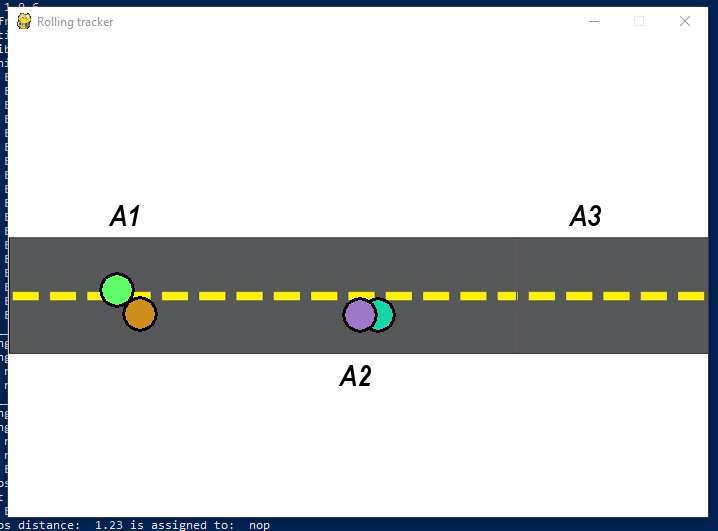
\includegraphics[width=0.7\textwidth]{../../Memmory/images/road_1.PNG}
                    \caption{Prueba piloto, carretera}
                    \label{fig:mesh11}
                \end{figure}
            \end{center}
        \subsubsection{Estabilidad del sistema}
            Tras esta primera prueba se optó por ver hasta que punto la tecnología es precisa, para lo cual se trazaron gráficas comparativas
            con los datos obtenidos a través de los equipos. En primer lugar se dejó durante un par de horas encendidos los equipos para ver las 
            fluctuaciones.
            \begin{center}
                \begin{figure}[]
                    \centering
                    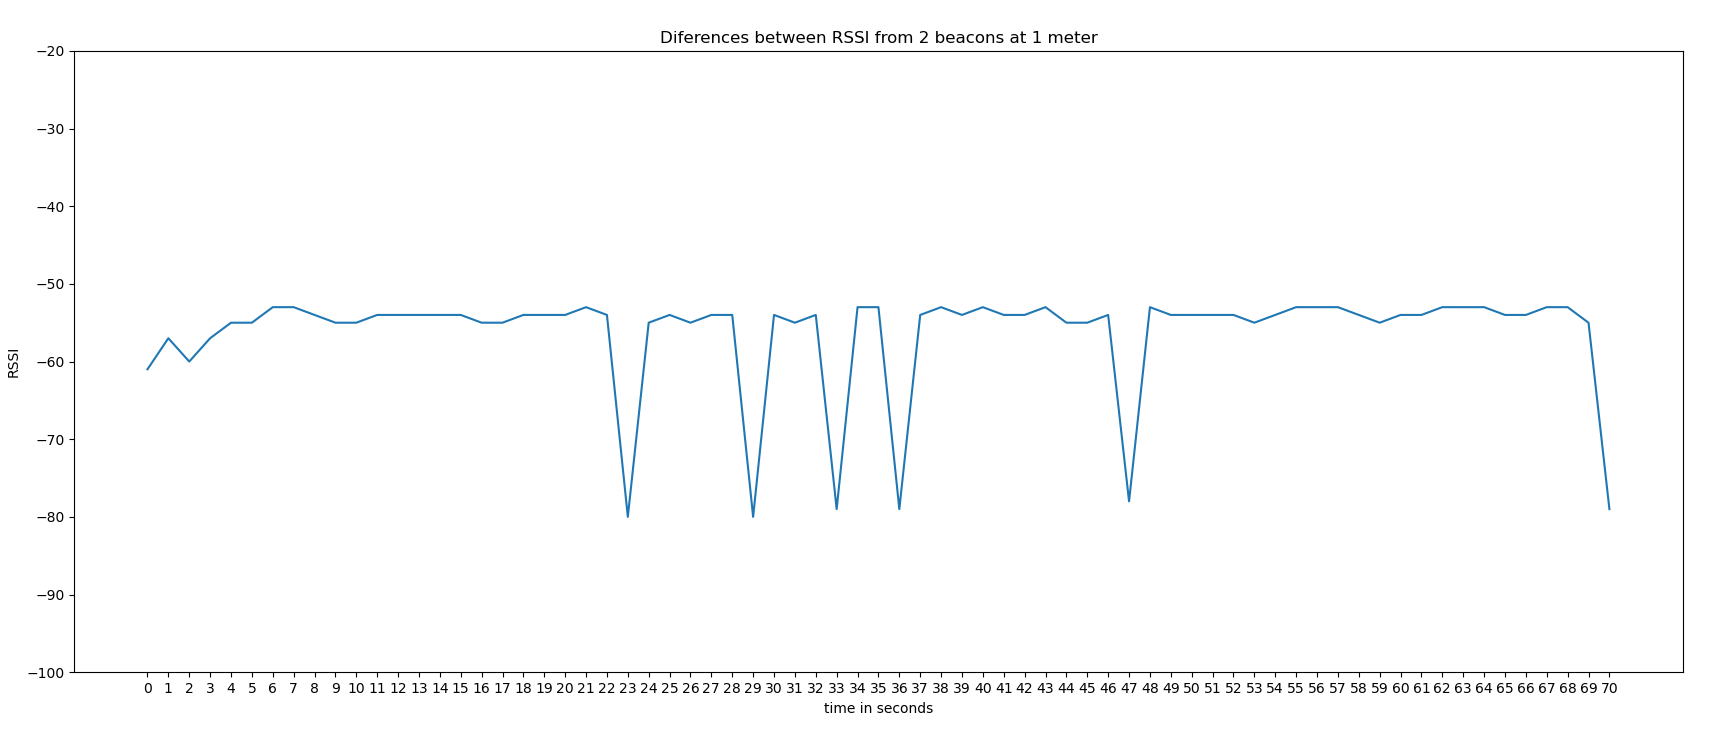
\includegraphics[width=1\textwidth]{../../Memmory/images/5min_beacon_rssi.PNG}
                    \caption{Toma de datos durante 2 horas}
                    \label{fig:mesh11}
                \end{figure}
            \end{center}
            Como podemos ver en la imagen las diferencias entre equipos estáticos son acusadas, es por ello por lo que queda demostrada la necesidad de
            desarrollar un filtro que anule este ruido radioeléctrico.
        \subsubsection{Posicionamiento real}
            El paso siguiente fue comprobar si tras filtrar las señales era realmente capaz de discernir si un Beacon se encontraba en una habitación
            o en otra tan solo atendiendo a su rssi, para lo cual se ha llevado a cabo una simulación que permite dibujar las dimensiones de las 
            habitaciones, la posición de los beacons e incluso el color de las mismas. 
            \begin{center}
                \begin{figure}[]
                    \centering
                    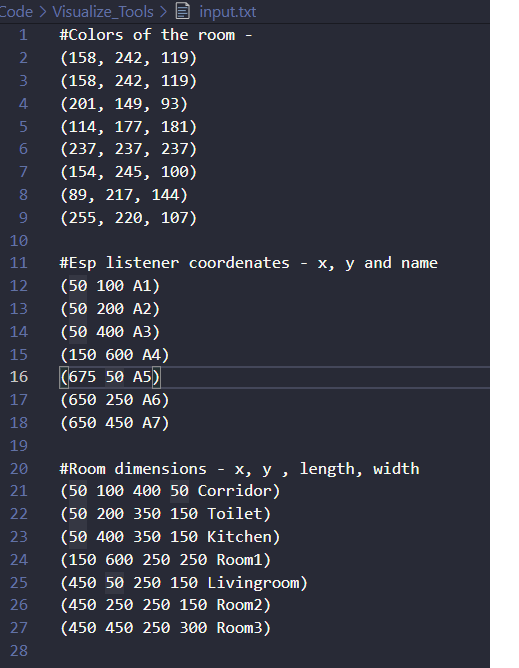
\includegraphics[width=0.5\textwidth]{../../Memmory/images/config_file_house.PNG}
                    \caption{Archivo de configuración de diseño de casa}
                    \label{fig:mesh11}
                \end{figure}
            \end{center}
            Una vez creada nuestra casa ya solo queda colocar realmente los equipos en lugares elevados y poco acesibles y ejecutar el script.
            Los equipos estuvieron durante una semana encendidos escuchando beacons y los resultados fueros los esperados.
            \begin{center}
                \begin{figure}[]
                    \centering
                    \includegraphics[width=0.5\textwidth]{../../Memmory/images/house_simulation_1.PNG}
                    \caption{Ejemplo de 3 personas dentro de una misma habitación}
                    \label{fig:mesh11}
                \end{figure}
            \end{center}          
            El caso más curioso de todos es que se dejaron beacons estáticos encima de armarios y la posición no móvil de los mismos 
            se mantuvo en la simulación en todo momento.
            \begin{center}
                \begin{figure}[]
                    \centering
                    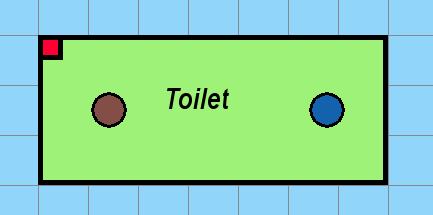
\includegraphics[width=0.5\textwidth]{../../Memmory/images/house_simulation_2.PNG}
                    \caption{Beacons estáticos durante la simulación}
                    \label{fig:mesh11}
                \end{figure}
            \end{center} 
            Al movernos dentro de la casa los masters de las habitaciones contiguas nos percibían con menor rssi, es por
            ello por lo que no nos visualizaba dentro de esa estancia.
            \begin{center}
                \begin{figure}[]
                    \centering
                    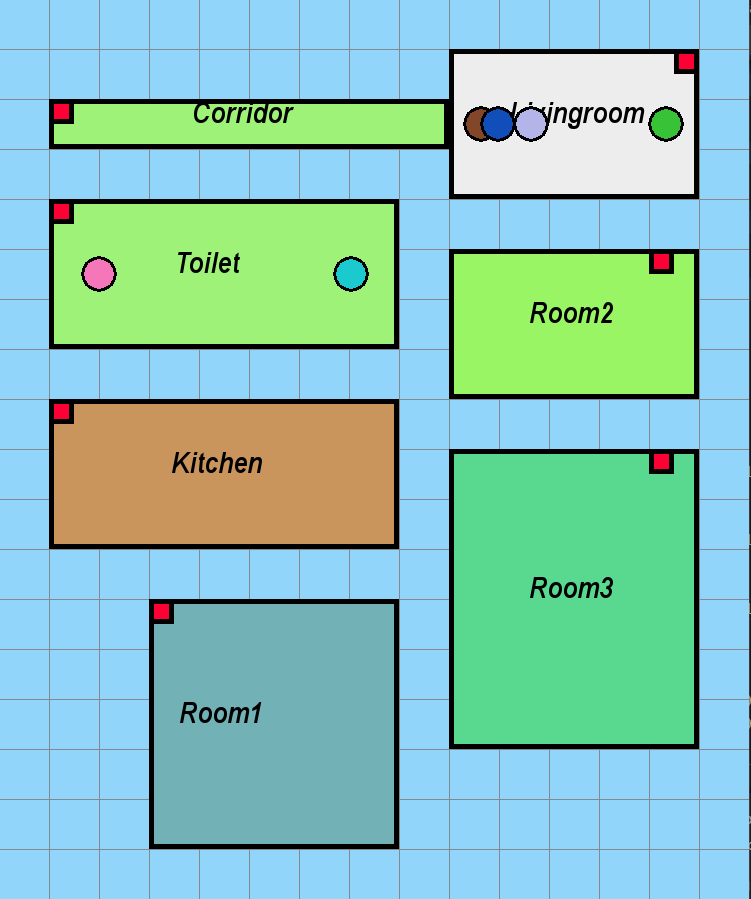
\includegraphics[width=0.5\textwidth]{../../Memmory/images/house_simulation_3.PNG}
                    \caption{Beacons en movimiento}
                    \label{fig:mesh11}
                \end{figure}
            \end{center}   
        \subsubsection{Prueba en supermercado}
            Una vez testada la tecnología se llevó a cabo una prueba real en un supermercado, para llevar a cabo la prueba
            se instalaron únicamente 2 masters y 6 beacons en carros en movimiento.
            Como suele pasar la prueba real no se parece tanto a las pruebas anteriores y podemos comprobar como 
            el algoritmo se complica más en asuncia de numerosos masters escuchando beacons, en este caso como solo se disponían
            de 2 los cálculos no siempre eran tan precisos y el filtro implementado en el caso de un desplazamiento rápido de un 
            equipo de punta a punta del supermercado no era el más óptimo.
            \begin{center}
                \begin{figure}[]
                    \centering
                    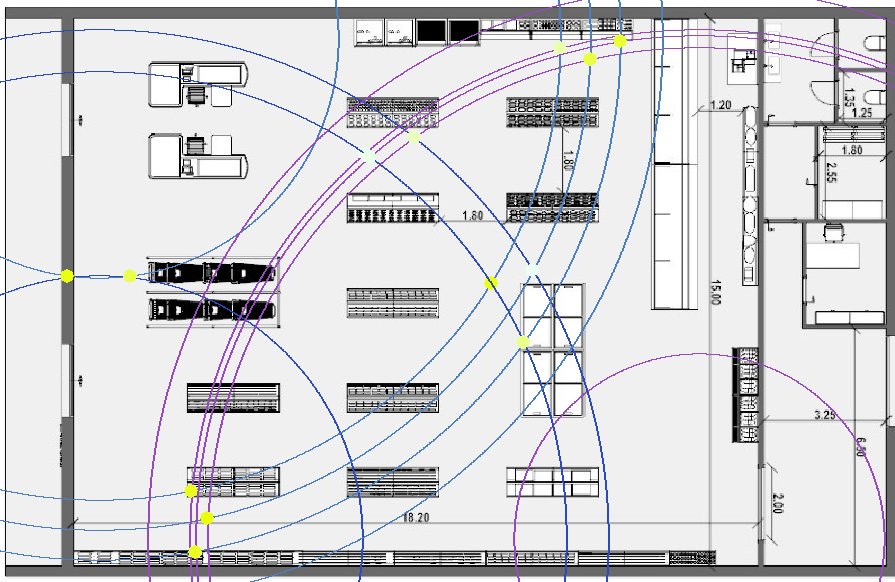
\includegraphics[width=0.7\textwidth]{../../Memmory/images/agrupation_3.PNG}
                    \caption{Beacons en movimiento dentro de supermercado captura 1}
                    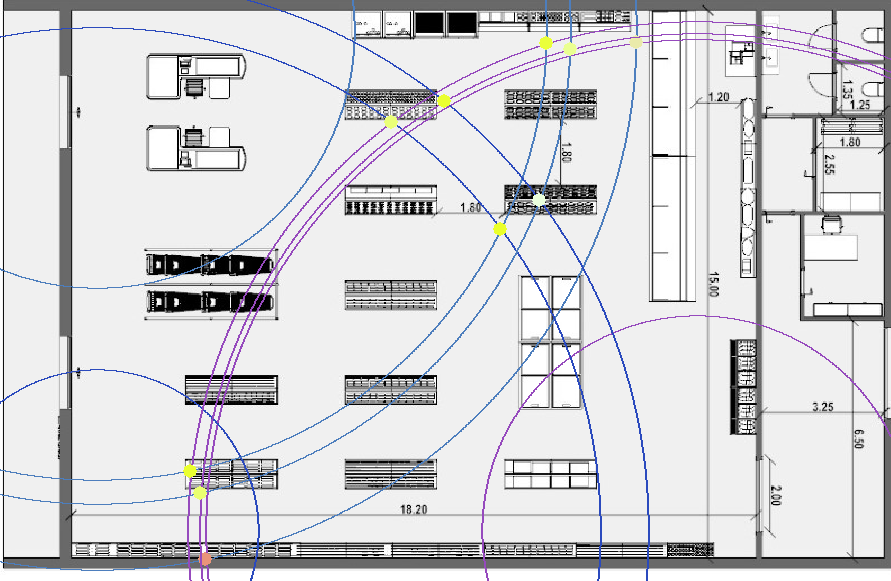
\includegraphics[width=0.7\textwidth]{../../Memmory/images/agrupation_2.PNG}
                    \caption{Beacons en movimiento dentro de supermercado captura 2}
                    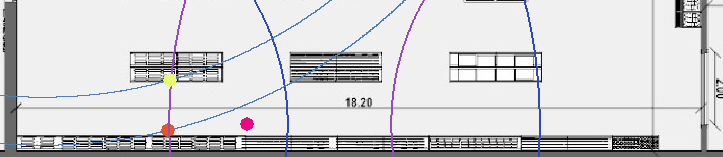
\includegraphics[width=0.5\textwidth]{../../Memmory/images/agrupation_1.PNG}
                    \caption{Beacons en supermercado percibidos solo por un master}
                    \label{fig:mesh11}
                \end{figure}
            \end{center}   
            
            Podemos ver como los puntos amarillos son los carros de la compra percibidos por ambos beacons y los rojos son aquellos
            que solo son escuchados por un master, de tal modo que le punto en el que se encuentran es menos precio.

\end{document} 